\documentclass[twoside]{book}

% Packages required by doxygen
\usepackage{fixltx2e}
\usepackage{calc}
\usepackage{doxygen}
\usepackage[export]{adjustbox} % also loads graphicx
\usepackage{graphicx}
\usepackage[utf8]{inputenc}
\usepackage{makeidx}
\usepackage{multicol}
\usepackage{multirow}
\PassOptionsToPackage{warn}{textcomp}
\usepackage{textcomp}
\usepackage[nointegrals]{wasysym}
\usepackage[table]{xcolor}

% Font selection
\usepackage[T1]{fontenc}
\usepackage[scaled=.90]{helvet}
\usepackage{courier}
\usepackage{amssymb}
\usepackage{sectsty}
\renewcommand{\familydefault}{\sfdefault}
\allsectionsfont{%
  \fontseries{bc}\selectfont%
  \color{darkgray}%
}
\renewcommand{\DoxyLabelFont}{%
  \fontseries{bc}\selectfont%
  \color{darkgray}%
}
\newcommand{\+}{\discretionary{\mbox{\scriptsize$\hookleftarrow$}}{}{}}

% Page & text layout
\usepackage{geometry}
\geometry{%
  a4paper,%
  top=2.5cm,%
  bottom=2.5cm,%
  left=2.5cm,%
  right=2.5cm%
}
\tolerance=750
\hfuzz=15pt
\hbadness=750
\setlength{\emergencystretch}{15pt}
\setlength{\parindent}{0cm}
\setlength{\parskip}{3ex plus 2ex minus 2ex}
\makeatletter
\renewcommand{\paragraph}{%
  \@startsection{paragraph}{4}{0ex}{-1.0ex}{1.0ex}{%
    \normalfont\normalsize\bfseries\SS@parafont%
  }%
}
\renewcommand{\subparagraph}{%
  \@startsection{subparagraph}{5}{0ex}{-1.0ex}{1.0ex}{%
    \normalfont\normalsize\bfseries\SS@subparafont%
  }%
}
\makeatother

% Headers & footers
\usepackage{fancyhdr}
\pagestyle{fancyplain}
\fancyhead[LE]{\fancyplain{}{\bfseries\thepage}}
\fancyhead[CE]{\fancyplain{}{}}
\fancyhead[RE]{\fancyplain{}{\bfseries\leftmark}}
\fancyhead[LO]{\fancyplain{}{\bfseries\rightmark}}
\fancyhead[CO]{\fancyplain{}{}}
\fancyhead[RO]{\fancyplain{}{\bfseries\thepage}}
\fancyfoot[LE]{\fancyplain{}{}}
\fancyfoot[CE]{\fancyplain{}{}}
\fancyfoot[RE]{\fancyplain{}{\bfseries\scriptsize Generated by Doxygen }}
\fancyfoot[LO]{\fancyplain{}{\bfseries\scriptsize Generated by Doxygen }}
\fancyfoot[CO]{\fancyplain{}{}}
\fancyfoot[RO]{\fancyplain{}{}}
\renewcommand{\footrulewidth}{0.4pt}
\renewcommand{\chaptermark}[1]{%
  \markboth{#1}{}%
}
\renewcommand{\sectionmark}[1]{%
  \markright{\thesection\ #1}%
}

% Indices & bibliography
\usepackage{natbib}
\usepackage[titles]{tocloft}
\setcounter{tocdepth}{3}
\setcounter{secnumdepth}{5}
\makeindex

% Hyperlinks (required, but should be loaded last)
\usepackage{ifpdf}
\ifpdf
  \usepackage[pdftex,pagebackref=true]{hyperref}
\else
  \usepackage[ps2pdf,pagebackref=true]{hyperref}
\fi
\hypersetup{%
  colorlinks=true,%
  linkcolor=blue,%
  citecolor=blue,%
  unicode%
}

% Custom commands
\newcommand{\clearemptydoublepage}{%
  \newpage{\pagestyle{empty}\cleardoublepage}%
}

\usepackage{caption}
\captionsetup{labelsep=space,justification=centering,font={bf},singlelinecheck=off,skip=4pt,position=top}

%===== C O N T E N T S =====

\begin{document}

% Titlepage & ToC
\hypersetup{pageanchor=false,
             bookmarksnumbered=true,
             pdfencoding=unicode
            }
\pagenumbering{alph}
\begin{titlepage}
\vspace*{7cm}
\begin{center}%
{\Large My Bike Game \\[1ex]\large v1.\+0 }\\
\vspace*{1cm}
{\large Generated by Doxygen 1.8.14}\\
\end{center}
\end{titlepage}
\clearemptydoublepage
\pagenumbering{roman}
\tableofcontents
\clearemptydoublepage
\pagenumbering{arabic}
\hypersetup{pageanchor=true}

%--- Begin generated contents ---
\chapter{File Index}
\section{File List}
Here is a list of all documented files with brief descriptions\+:\begin{DoxyCompactList}
\item\contentsline{section}{Coursework 2 -\/ starter/\+Coursework 2 -\/ starter/include/\mbox{\hyperlink{_background_8h}{Background.\+h}} }{\pageref{_background_8h}}{}
\item\contentsline{section}{Coursework 2 -\/ starter/\+Coursework 2 -\/ starter/include/\mbox{\hyperlink{_bike_8h}{Bike.\+h}} }{\pageref{_bike_8h}}{}
\item\contentsline{section}{Coursework 2 -\/ starter/\+Coursework 2 -\/ starter/include/\mbox{\hyperlink{_block_shape_8h}{Block\+Shape.\+h}} }{\pageref{_block_shape_8h}}{}
\item\contentsline{section}{Coursework 2 -\/ starter/\+Coursework 2 -\/ starter/include/{\bfseries Definitions.\+h} }{\pageref{_definitions_8h}}{}
\item\contentsline{section}{Coursework 2 -\/ starter/\+Coursework 2 -\/ starter/include/\mbox{\hyperlink{_game_8h}{Game.\+h}} }{\pageref{_game_8h}}{}
\item\contentsline{section}{Coursework 2 -\/ starter/\+Coursework 2 -\/ starter/include/{\bfseries Joint.\+h} }{\pageref{_joint_8h}}{}
\item\contentsline{section}{Coursework 2 -\/ starter/\+Coursework 2 -\/ starter/include/\mbox{\hyperlink{_level_loader_8h}{Level\+Loader.\+h}} }{\pageref{_level_loader_8h}}{}
\item\contentsline{section}{Coursework 2 -\/ starter/\+Coursework 2 -\/ starter/include/\mbox{\hyperlink{_line_8h}{Line.\+h}} }{\pageref{_line_8h}}{}
\item\contentsline{section}{Coursework 2 -\/ starter/\+Coursework 2 -\/ starter/include/\mbox{\hyperlink{_physical_object_8h}{Physical\+Object.\+h}} }{\pageref{_physical_object_8h}}{}
\item\contentsline{section}{Coursework 2 -\/ starter/\+Coursework 2 -\/ starter/include/\mbox{\hyperlink{_screen_text_8h}{Screen\+Text.\+h}} }{\pageref{_screen_text_8h}}{}
\end{DoxyCompactList}

\chapter{File Documentation}
\hypertarget{_background_8h}{}\section{Coursework 2 -\/ starter/\+Coursework 2 -\/ starter/include/\+Background.h File Reference}
\label{_background_8h}\index{Coursework 2 -\/ starter/\+Coursework 2 -\/ starter/include/\+Background.\+h@{Coursework 2 -\/ starter/\+Coursework 2 -\/ starter/include/\+Background.\+h}}
{\ttfamily \#include $<$S\+F\+M\+L/\+Graphics.\+hpp$>$}\newline
Include dependency graph for Background.\+h\+:\nopagebreak
\begin{figure}[H]
\begin{center}
\leavevmode
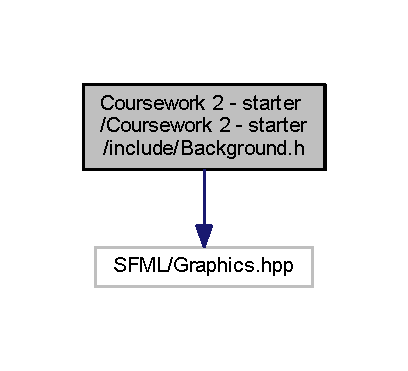
\includegraphics[width=196pt]{_background_8h__incl}
\end{center}
\end{figure}
This graph shows which files directly or indirectly include this file\+:\nopagebreak
\begin{figure}[H]
\begin{center}
\leavevmode
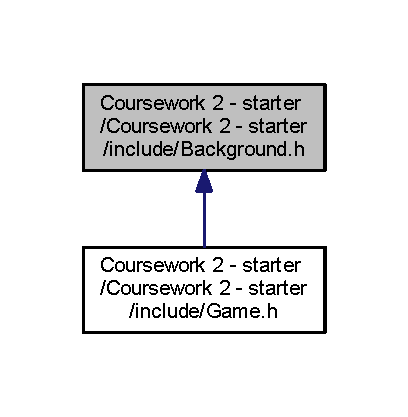
\includegraphics[width=196pt]{_background_8h__dep__incl}
\end{center}
\end{figure}


\subsection{Detailed Description}
This class builds a fixed background, and because of that it doesnt really pass many arguments or have any special reuseability to it, its kind of just a seperate class that builds once instance of a background.

If I did not struggle with some things I would spend time passing these backgrounds in thorugh file. 
\hypertarget{_bike_8h}{}\section{Coursework 2 -\/ starter/\+Coursework 2 -\/ starter/include/\+Bike.h File Reference}
\label{_bike_8h}\index{Coursework 2 -\/ starter/\+Coursework 2 -\/ starter/include/\+Bike.\+h@{Coursework 2 -\/ starter/\+Coursework 2 -\/ starter/include/\+Bike.\+h}}
{\ttfamily \#include $<$Box2\+D/\+Box2\+D.\+h$>$}\newline
{\ttfamily \#include $<$S\+F\+M\+L/\+Graphics.\+hpp$>$}\newline
{\ttfamily \#include \char`\"{}Physical\+Object.\+h\char`\"{}}\newline
Include dependency graph for Bike.\+h\+:\nopagebreak
\begin{figure}[H]
\begin{center}
\leavevmode

\includegraphics[width=350pt]{_bike_8h__incl}
\end{center}
\end{figure}
This graph shows which files directly or indirectly include this file\+:\nopagebreak
\begin{figure}[H]
\begin{center}
\leavevmode
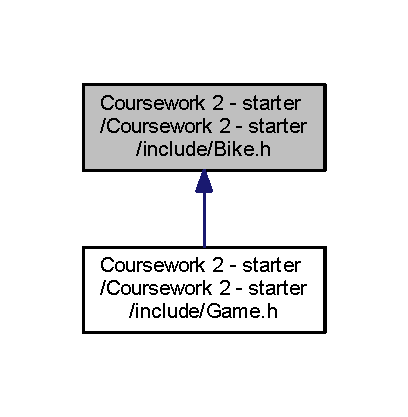
\includegraphics[width=196pt]{_bike_8h__dep__incl}
\end{center}
\end{figure}
\subsection*{Macros}
\begin{DoxyCompactItemize}
\item 
\mbox{\Hypertarget{_bike_8h_af7e8592d0a634bd3642e9fd508ea8022}\label{_bike_8h_af7e8592d0a634bd3642e9fd508ea8022}} 
\#define {\bfseries D\+E\+G2\+R\+AD}~0.\+017453f;
\item 
\mbox{\Hypertarget{_bike_8h_ac5a945020d3528355cda82d383676736}\label{_bike_8h_ac5a945020d3528355cda82d383676736}} 
\#define {\bfseries R\+A\+D2\+D\+EG}~57.\+29577f;
\end{DoxyCompactItemize}


\subsection{Detailed Description}
The bike class that essentially builds a bike from different bodies and sfml drawings.

This class is not very object oriented in terms of reuseability. On the contrary its a very complex class with many different things added to it and is not really meant for building differently.

If I where to do different type of player cars I would probably restructure it a little bit in terms of loading in sprites from file etc. 
\hypertarget{_block_shape_8h}{}\section{Coursework 2 -\/ starter/\+Coursework 2 -\/ starter/include/\+Block\+Shape.h File Reference}
\label{_block_shape_8h}\index{Coursework 2 -\/ starter/\+Coursework 2 -\/ starter/include/\+Block\+Shape.\+h@{Coursework 2 -\/ starter/\+Coursework 2 -\/ starter/include/\+Block\+Shape.\+h}}
{\ttfamily \#include $<$Box2\+D/\+Box2\+D.\+h$>$}\newline
{\ttfamily \#include $<$S\+F\+M\+L/\+Graphics.\+hpp$>$}\newline
{\ttfamily \#include \char`\"{}Physical\+Object.\+h\char`\"{}}\newline
Include dependency graph for Block\+Shape.\+h\+:\nopagebreak
\begin{figure}[H]
\begin{center}
\leavevmode
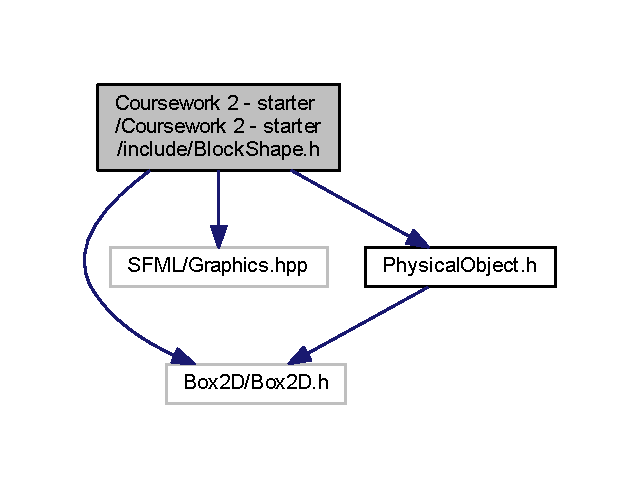
\includegraphics[width=307pt]{_block_shape_8h__incl}
\end{center}
\end{figure}
This graph shows which files directly or indirectly include this file\+:\nopagebreak
\begin{figure}[H]
\begin{center}
\leavevmode
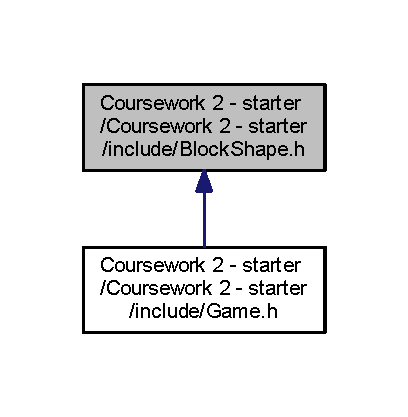
\includegraphics[width=196pt]{_block_shape_8h__dep__incl}
\end{center}
\end{figure}
\subsection*{Macros}
\begin{DoxyCompactItemize}
\item 
\mbox{\Hypertarget{_block_shape_8h_af7e8592d0a634bd3642e9fd508ea8022}\label{_block_shape_8h_af7e8592d0a634bd3642e9fd508ea8022}} 
\#define {\bfseries D\+E\+G2\+R\+AD}~0.\+017453f;
\item 
\mbox{\Hypertarget{_block_shape_8h_ac5a945020d3528355cda82d383676736}\label{_block_shape_8h_ac5a945020d3528355cda82d383676736}} 
\#define {\bfseries R\+A\+D2\+D\+EG}~57.\+29577f;
\end{DoxyCompactItemize}


\subsection{Detailed Description}
This class has some simple block body and drawing.

it currently draws and creates one block in the world and updates it.

This class was created to make some building blocks that would act as obstacles or similiary, due to other issues I had to pause this part of the project and just leave it as an OO class that has a decent block shape with reuseability when I would need it ni the future. 
\hypertarget{_game_8h}{}\section{Coursework 2 -\/ starter/\+Coursework 2 -\/ starter/include/\+Game.h File Reference}
\label{_game_8h}\index{Coursework 2 -\/ starter/\+Coursework 2 -\/ starter/include/\+Game.\+h@{Coursework 2 -\/ starter/\+Coursework 2 -\/ starter/include/\+Game.\+h}}
{\ttfamily \#include $<$Box2\+D/\+Box2\+D.\+h$>$}\newline
{\ttfamily \#include $<$S\+F\+M\+L/\+Audio/\+Music.\+hpp$>$}\newline
{\ttfamily \#include $<$S\+F\+M\+L/\+Graphics.\+hpp$>$}\newline
{\ttfamily \#include \char`\"{}Line.\+h\char`\"{}}\newline
{\ttfamily \#include \char`\"{}Bike.\+h\char`\"{}}\newline
{\ttfamily \#include \char`\"{}Background.\+h\char`\"{}}\newline
{\ttfamily \#include \char`\"{}Block\+Shape.\+h\char`\"{}}\newline
{\ttfamily \#include \char`\"{}Bridge.\+h\char`\"{}}\newline
{\ttfamily \#include \char`\"{}Screen\+Text.\+h\char`\"{}}\newline
Include dependency graph for Game.\+h\+:
\nopagebreak
\begin{figure}[H]
\begin{center}
\leavevmode

\includegraphics[width=350pt]{_game_8h__incl}
\end{center}
\end{figure}


\subsection{Detailed Description}
The main game loop.

This class draws, sets the view, updates the screen and processes key presses and more. This class holds all the game logic, 
\hypertarget{_level_loader_8h}{}\section{Coursework 2 -\/ starter/\+Coursework 2 -\/ starter/include/\+Level\+Loader.h File Reference}
\label{_level_loader_8h}\index{Coursework 2 -\/ starter/\+Coursework 2 -\/ starter/include/\+Level\+Loader.\+h@{Coursework 2 -\/ starter/\+Coursework 2 -\/ starter/include/\+Level\+Loader.\+h}}
{\ttfamily \#include $<$stdio.\+h$>$}\newline
{\ttfamily \#include $<$string$>$}\newline
{\ttfamily \#include $<$vector$>$}\newline
{\ttfamily \#include $<$iostream$>$}\newline
{\ttfamily \#include $<$fstream$>$}\newline
{\ttfamily \#include $<$sstream$>$}\newline
Include dependency graph for Level\+Loader.\+h\+:\nopagebreak
\begin{figure}[H]
\begin{center}
\leavevmode
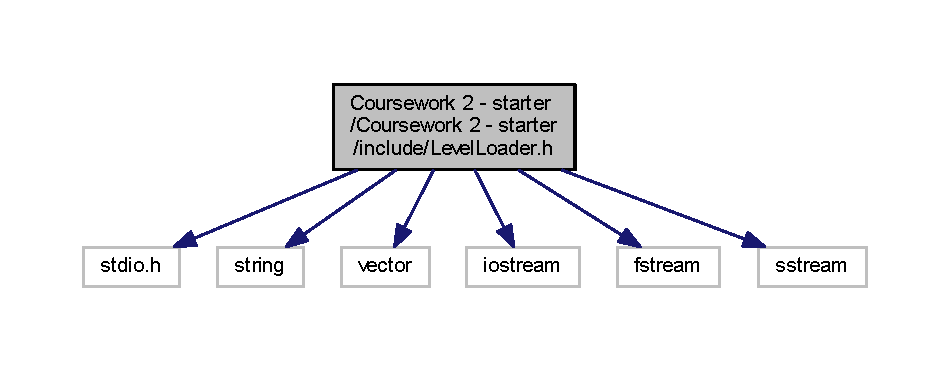
\includegraphics[width=350pt]{_level_loader_8h__incl}
\end{center}
\end{figure}
This graph shows which files directly or indirectly include this file\+:\nopagebreak
\begin{figure}[H]
\begin{center}
\leavevmode
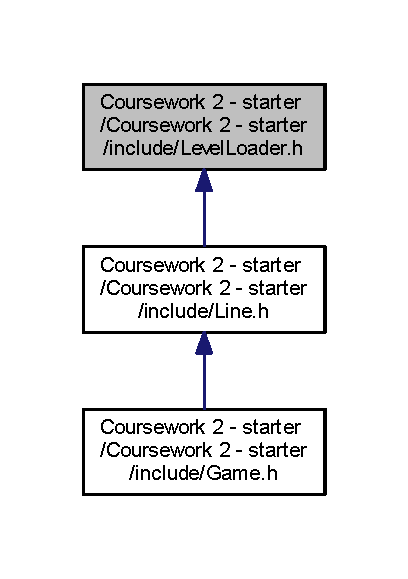
\includegraphics[width=196pt]{_level_loader_8h__dep__incl}
\end{center}
\end{figure}


\subsection{Detailed Description}
Loads in points in world through file

This class loads in a set of points in the world through file

This class uses the Singleton design pattern. 
\hypertarget{_line_8h}{}\section{Coursework 2 -\/ starter/\+Coursework 2 -\/ starter/include/\+Line.h File Reference}
\label{_line_8h}\index{Coursework 2 -\/ starter/\+Coursework 2 -\/ starter/include/\+Line.\+h@{Coursework 2 -\/ starter/\+Coursework 2 -\/ starter/include/\+Line.\+h}}
{\ttfamily \#include $<$Box2\+D/\+Box2\+D.\+h$>$}\newline
{\ttfamily \#include $<$S\+F\+M\+L/\+Graphics.\+hpp$>$}\newline
{\ttfamily \#include $<$iostream$>$}\newline
{\ttfamily \#include \char`\"{}..\textbackslash{}include\textbackslash{}\+Level\+Loader.\+h\char`\"{}}\newline
Include dependency graph for Line.\+h\+:\nopagebreak
\begin{figure}[H]
\begin{center}
\leavevmode
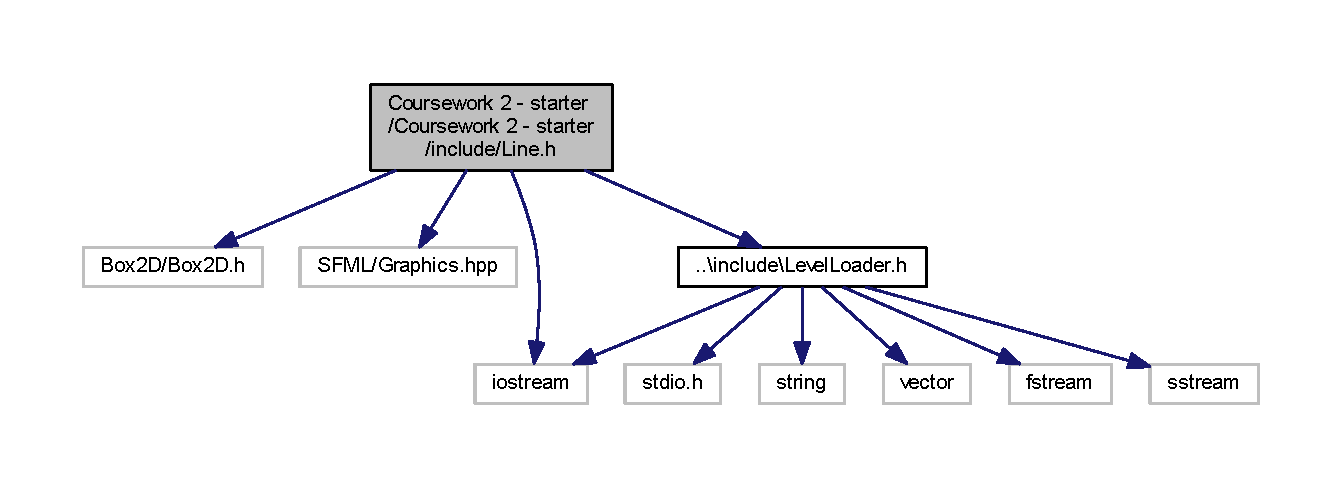
\includegraphics[width=350pt]{_line_8h__incl}
\end{center}
\end{figure}
This graph shows which files directly or indirectly include this file\+:\nopagebreak
\begin{figure}[H]
\begin{center}
\leavevmode
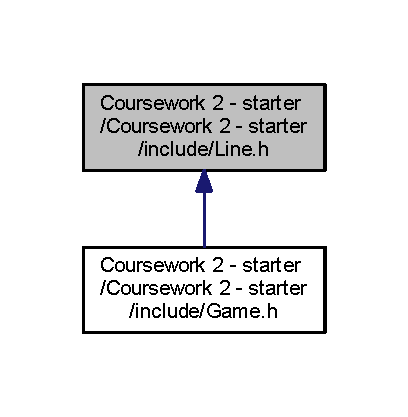
\includegraphics[width=196pt]{_line_8h__dep__incl}
\end{center}
\end{figure}


\subsection{Detailed Description}
This class draws and sets the line in the world.

This line is specifically used for acting as the ground which the player will drive around on with the bike. This class takes x amount of floats and sets them as vertices, it also creates a box2d chain object and draws an sfml line .the positions are loaded in from file to make it kind of easier to construct the level. the file reads two vertices and sets them as the line and draws them in random colour to give it a funky space look. 
\hypertarget{_physical_object_8h}{}\section{Coursework 2 -\/ starter/\+Coursework 2 -\/ starter/include/\+Physical\+Object.h File Reference}
\label{_physical_object_8h}\index{Coursework 2 -\/ starter/\+Coursework 2 -\/ starter/include/\+Physical\+Object.\+h@{Coursework 2 -\/ starter/\+Coursework 2 -\/ starter/include/\+Physical\+Object.\+h}}
{\ttfamily \#include $<$Box2\+D/\+Box2\+D.\+h$>$}\newline
Include dependency graph for Physical\+Object.\+h\+:\nopagebreak
\begin{figure}[H]
\begin{center}
\leavevmode
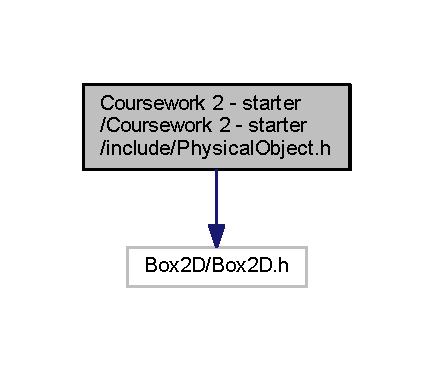
\includegraphics[width=208pt]{_physical_object_8h__incl}
\end{center}
\end{figure}
This graph shows which files directly or indirectly include this file\+:\nopagebreak
\begin{figure}[H]
\begin{center}
\leavevmode
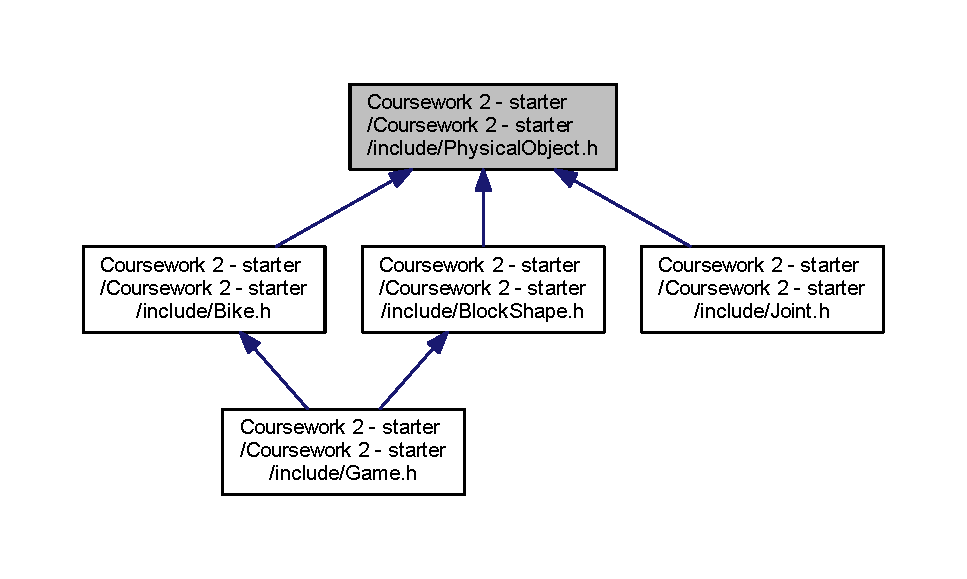
\includegraphics[width=350pt]{_physical_object_8h__dep__incl}
\end{center}
\end{figure}
\subsection*{Macros}
\begin{DoxyCompactItemize}
\item 
\mbox{\Hypertarget{_physical_object_8h_af7e8592d0a634bd3642e9fd508ea8022}\label{_physical_object_8h_af7e8592d0a634bd3642e9fd508ea8022}} 
\#define {\bfseries D\+E\+G2\+R\+AD}~0.\+017453f;
\item 
\mbox{\Hypertarget{_physical_object_8h_ac5a945020d3528355cda82d383676736}\label{_physical_object_8h_ac5a945020d3528355cda82d383676736}} 
\#define {\bfseries R\+A\+D2\+D\+EG}~57.\+29577f;
\end{DoxyCompactItemize}


\subsection{Detailed Description}
Class that defines degrees and radians

degrees to radians,radians to degrees 
\hypertarget{_screen_text_8h}{}\section{Coursework 2 -\/ starter/\+Coursework 2 -\/ starter/include/\+Screen\+Text.h File Reference}
\label{_screen_text_8h}\index{Coursework 2 -\/ starter/\+Coursework 2 -\/ starter/include/\+Screen\+Text.\+h@{Coursework 2 -\/ starter/\+Coursework 2 -\/ starter/include/\+Screen\+Text.\+h}}
{\ttfamily \#include $<$S\+F\+M\+L/\+Graphics.\+hpp$>$}\newline
Include dependency graph for Screen\+Text.\+h\+:\nopagebreak
\begin{figure}[H]
\begin{center}
\leavevmode
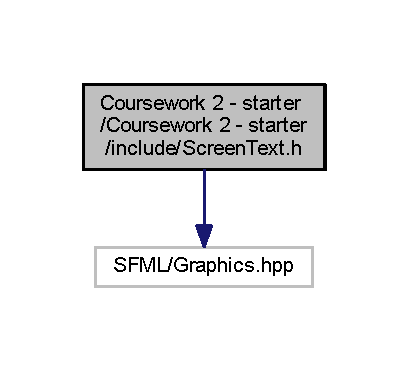
\includegraphics[width=196pt]{_screen_text_8h__incl}
\end{center}
\end{figure}
This graph shows which files directly or indirectly include this file\+:\nopagebreak
\begin{figure}[H]
\begin{center}
\leavevmode
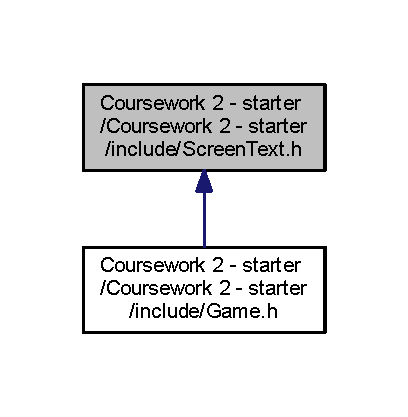
\includegraphics[width=196pt]{_screen_text_8h__dep__incl}
\end{center}
\end{figure}


\subsection{Detailed Description}
Class that draws text to the screen

This class is currently supposed to keep track of score and win conditions etc.

This class was created to give a nice OO design and reuseability for drawing text to the screen, such as player score and menu text. 
%--- End generated contents ---

% Index
\backmatter
\newpage
\phantomsection
\clearemptydoublepage
\addcontentsline{toc}{chapter}{Index}
\printindex

\end{document}
